%==============================================================================
%== template for LATEX poster =================================================
%==============================================================================
%
%--A0 beamer slide-------------------------------------------------------------
\documentclass[final]{beamer} % use beamer
\usepackage[orientation=portrait,
            size=a0,          % poster size
            scale=1.15        % font scale factor
           ]{beamerposter}    % beamer in poster size
%
%--some needed packages--------------------------------------------------------
\usepackage[english]{babel}  % language 
\usepackage[utf8]{inputenc}   % std linux encoding
\usepackage{multicol}
\usepackage{amsmath,amsthm, amssymb, latexsym} 
\usepackage{graphicx}
\usepackage{natbib}
% Beamer doesn't have \newblock defined which natbib needs.  Define our own:
\def\newblock{\hskip .11em plus .33em minus 0.07em}
%
%==The poster style============================================================
\usetheme{tycposter}            % our poster style
%--set colors for blocks (without frame)---------------------------------------
  \setbeamercolor{block title}{fg=mgreen,bg=white}
  \setbeamercolor{block body}{fg=black,bg=white}
%--set colors for alerted blocks (with frame)----------------------------------
%--textcolor = fg, backgroundcolor = bg, dblue is the jacobs blue
  \setbeamercolor{block alerted title}{fg=white,bg=tycblue!70}%frame color
  \setbeamercolor{block alerted body}{fg=black,bg=tycblue!10}%body color
  \setlength{\columnsep}{36pt}
%
%==Titel, date and authors of the poster=======================================
\title{Experiments with the Full Configuration Interaction Quantum Monte Carlo method}
\author{J.S.~Spencer\inst{1,2}, J.~Weston\inst{2} and W.M.C.~Foulkes\inst{2}}
\institute[Imperial College London]
          {\inst{1}Thomas Young Centre, Imperial College London, U.K.\\
          \inst{2}Department of Physics, Imperial College London, U.K.}
\date{\today}
%
%==some usefull qm commands====================================================
%  |x>
\newcommand{\ket}[1]{\left\vert#1\right\rangle}
%  <x|
\newcommand{\bra}[1]{\left\langle#1\right\vert}
%  <x|y>
\newcommand{\braket}[2]{\left< #1 \vphantom{#2}\,
                        \right\vert\left.\!\vphantom{#1} #2 \right>}
%  <x|a|y>
\newcommand{\sandwich}[3]{\left< #1 \vphantom{#2 #3} \right|
                          #2 \left|\vphantom{#1 #2} #3 \right>}
%  Dy/Dx
\newcommand{\pdd}[2]{\frac{\partial#1}{\partial#2}}
%  |x|
\newcommand{\abs}[1]{\left\vert#1\right\vert}
% < x >
\newcommand{\mean}[1]{\langle#1\rangle}
%  k_{x}
\newcommand{\kv}[1]{\mathbf{k}_{#1}}
% H
\newcommand{\Hamil}{\hat{H}}
% O
\newcommand{\Op}{\hat{O}}
% FCIQMC
\newcommand{\Dz}{D_\mathbf{0}}
\newcommand{\dt}{\delta\tau}
\newcommand{\pgen}{p_{\textrm{gen}}}
\newcommand{\Emax}{E_{\textrm{max}}}
% vectors...
\newcommand{\bz}{\mathbf{0}}
\newcommand{\bi}{\mathbf{i}}
\newcommand{\bj}{\mathbf{j}}
\newcommand{\cc}{\mathbf{c}}
% matrices...
\newcommand{\HH}{\mathbf{H}}
\newcommand{\II}{\mathbf{I}}
%==============================================================================
%==the poster content==========================================================
%==============================================================================
\begin{document}
% The poster is one beamer frame, so we have to start with:
\begin{frame}[t]
% Hack margins: enclose everything in a single column which is 90% of the width
% of the entire page.
\begin{columns}[t]
\begin{column}{0.9\paperwidth}
%
% Start for real!
%
   \begin{alertblock}{Introduction}
       \begin{multicols}{3}
           The Full Configuration Interaction energy of a system can be obtained through diagonalisation of the Hamiltonian matrix and gives the exact solution to the Schr\"odinger equation within the basis set used.  However, the cost of an FCI calculation grows exponentially with system size.
           
           A new quantum Monte Carlo method, called Full Configuration Interaction Quantum Monte Carlo (FCIQMC)\cite{booth:2009}, has recently been proposed which enables the FCI result to be obtained stochastically.  FCIQMC has been used to perform FCI-quality calculations on many systems which were previously impossible\cite{booth:2009,booth:2010}.  Recent developments\cite{cleland:2010} indicate that FCIQMC might be applicable to even larger systems. 
       \end{multicols}
   \end{alertblock}
%
   \begin{block}{Full Configuration Interaction Quantum Monte Carlo}
%
       \begin{multicols}{3}
           In a similar fashion to Diffusion Monte Carlo, FCIQMC simulates the imaginary-time Schr\"odinger equation by stochastically evolving a population of ``psips'', which propagate throughout the Hilbert space.  However, unlike DMC, FCIQMC imposes no sign structure on the wavefunction.

           The imaginary-time Schr\"odinger equation is:
           \begin{equation}
               \pdd{\Psi}{\tau} = - \Hamil \Psi.
           \end{equation}
           The long-time integration of an initial function, $\Dz$, gives the ground state wavefunction
           \begin{equation}
               \Psi_\bz = \lim_{\tau\rightarrow\infty} e^{-\tau(\Hamil -E_\bz)} \Dz.
           \end{equation}
           By expressing the wavefunction as a linear combination of Slater determinants, $\{D_\bi\}$, which are antisymmetric by construction, only fermionic solutions can be found:
           \begin{equation}
               \Psi(\tau) = \sum_\bi c_\bi(\tau) \ket{D_\bi}.
           \end{equation}
           A diffusion equation for the coefficients, $\{c_\bi\}$, is obtained by substituting the expansion into the time-dependent Schr\"odinger equation:
           \begin{equation}
               \pdd{c_\bi(\tau)}{\tau} = -\sum_\bj (H_{\bi\bj} -S\delta_{\bi\bj}) c_\bj(\tau)
           \end{equation}
           where $S$ is a arbitrary energy ``shift'' (analogous to that in DMC) which controls the total population of psips.  The coefficient $c_\bi$ is proportional to a signed sum of psips on determinant $D_\bi$, and so the psips can be evolved by following the discretized diffusion equation.

           The psip population is propagated at each timestep, $\dt$, in three stages:
           \begin{enumerate}
           \item Spawning

           Each psip attempts to spawn from its own location, $D_\bi$, onto a connected determinant, $D_\bj, \bj\ne\bi$, which is randomly selected with a normalised probability, $\pgen(\bj|\bi)$.  The attempted spawning is accepted with probability
           \begin{equation}
               p_{\textrm{spawn}}(\bj|\bi) = \frac{\dt\abs{H_{\bi\bj}}}{\pgen(\bj|\bi)}
           \end{equation}

           If $H_{\bi\bj}$ is positive, then the child psip will have the opposite sign to its parent, otherwise the child will have the same sign.
           \item Cloning/Death

           Each psip attempts to clone itself or die with probability
           \begin{equation}
               p_{\textrm{death}}(\bi) = \dt\abs{H_{\bi\bi}-S}.
           \end{equation}
           The change in population (i.e. whether cloning or death occurs) is determined by the sign of $S-H_{\bi\bi}$.
           \item Annihilation

           After all psips have attempted to spawn and clone/die, psips residing on the same determinant are gathered together and those of opposite sign cancel out.  This step is crucial in preventing an exponential growth of noise in the system.
           \end{enumerate}
           \begin{center}
           \begin{minipage}{\columnwidth}
           \begin{block}{Timestep errors}
               Each iteration uses the propagator $\II - (\HH - S\II)\dt$ instead of the exact propagator, $\exp(-(\HH - S\II)\dt)$.  If \mbox{$\dt \leq 2/(\Emax - E_0)$}, where $\Emax$ is the highest energy state and $E_0$ is the ground state energy, then both propagators lead to the exact ground state.  In practice $\dt$ is much smaller than this limit to avoid excessive noise in the population dynamics and so timestep errors do not occur.
           \end{block}
           \end{minipage}
           \end{center}
       \end{multicols}
%
       \begin{columns}[t]
           \begin{column}{0.74\paperwidth}
               \begin{alertblock}{Energy estimators}
               \begin{multicols}{2}
               The energy is measured during a simulation via two different estimators.  The shift is updated every $A$ iterations according to
               \begin{equation}
                   S(\tau) = S(\tau - A\dt) - \frac{\zeta}{A\dt}\ln\frac{N_p(\tau)}{N_p(\tau-A\dt)}
               \end{equation}
               If the psip population, $N_p$, is constant, then $\HH\cc = S\cc$.

               The energy can also be estimated via a projection:
               \begin{equation}
                  E(\tau) = \sum_\bj \bra{D_\bz}\Hamil\ket{D_\bj} \frac{N_\bj(\tau)}{N_\bz(\tau)}.
               \end{equation}

               $\bra{\Dz}\Hamil\ket{\Dz}$ is usually subtracted from the diagonal Hamiltonian matrix elements and so $S$ and $E$ give the correlation energy.
               \end{multicols}
               % Ensure end matches up with Averages quantities.
               \vspace{-0.22cm}
               \end{alertblock}
           \end{column}
           \begin{column}{0.16\paperwidth}
               \begin{alertblock}{Averaged quantities}
               It is important to note that $\mean{N_\bj/N_\bz} \ne \mean{N_\bj}/\mean{N_\bz}$.  
               
               Hence to obtain the average of the projected energy, $\sum_\bj \bra{D_\bj}\Hamil\ket{\Dz} N_\bj$ and $N_\bz$ must be averaged separately.
               \end{alertblock}
           \end{column}
       \end{columns}
%
   \end{block}
%
   \begin{block}{Population dynamics: the 12-site 1D Hubbard model at $U=2t$}
       \begin{multicols}{4}
          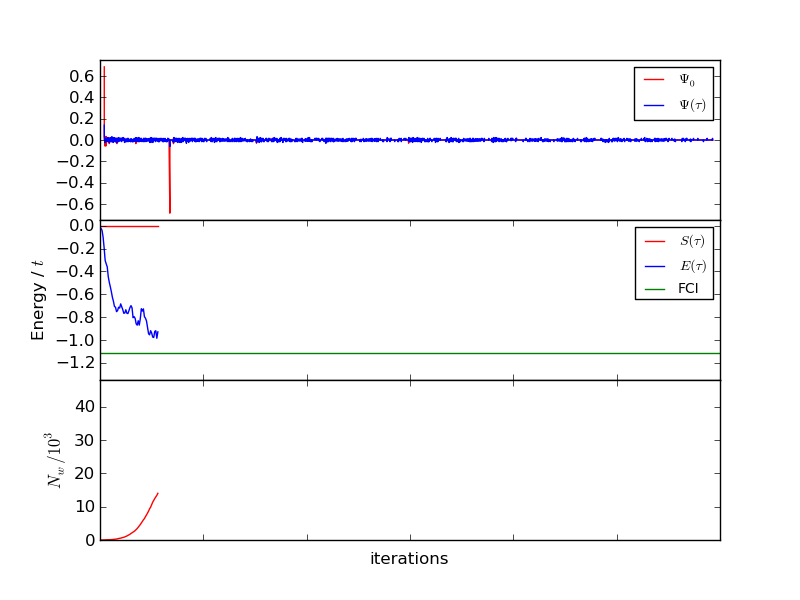
\includegraphics[width=0.95\linewidth]{step055}

          The population grows rapidly from a psip on \columnbreak $\Dz$ and spreads throughout the space.
          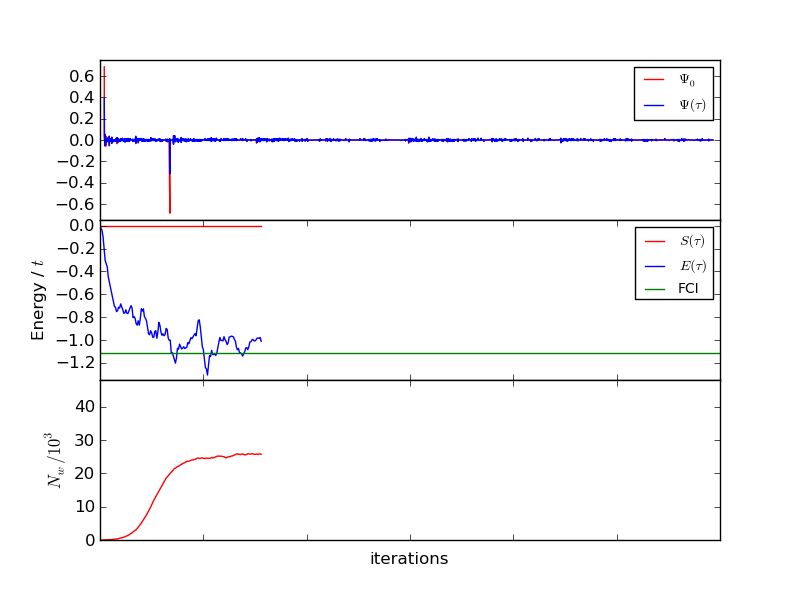
\includegraphics[width=0.95\linewidth]{step155}

          The sign structure of the wavefunction emerges \columnbreak during a plateau in the psip growth.
          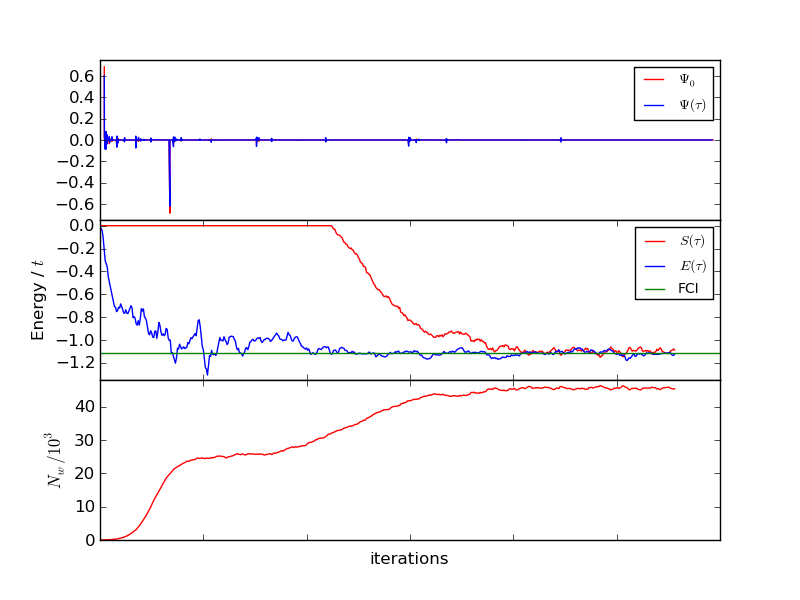
\includegraphics[width=0.95\linewidth]{step555}

          The psips now model the exact wavefunction.  The \columnbreak shift quickly converges to the FCI energy.

         This behaviour occurs in almost all systems that have been studied.  The plateau height varies with system, but (at least for molecular systems) is less than the size of the space.  After the plateau the population is stabilised by allowing the shift to vary.  Unfortunately the plateau height for the Hubbard model quickly exceeds the size of the space as $U$ increases and we are currently limited to systems which FCI can also handle.  We are attempting to understand why this occurs and hope that the Hubbard model will serve as a testing ground for theoretical developments.
       \end{multicols}
   \end{block}
% 
   \begin{columns}[t]
%
       \begin{column}{0.33\paperwidth}
           \begin{block}{A continuous-time algorithm}
           The timestep used in FCIQMC means that the probability of a spawning event occurring during an iteration is very small and the rejected spawning events are a waste of CPU time.  We have formulated a continuous-time algorithm which ``jumps'' directly to the next spawning event.  Defining $R_{\bi\bj} = \abs{H_{\bi\bj}-S\delta_{\bi\bj}}$ and $R_\bi = \sum_\bj R_{\bi\bj}$, the psip population can be evolved as follows:
           \begin{itemize}
           \item Select the time of the next spawning event from a psip on $D_\bi$ according to the probability distribution function $R_\bi e^{-R_\bi t}$.  The p.d.f.~follows from the probability of spawning a child from a psip on $D_\bi$ onto $D_\bj$ in time $\Delta t$ is $R_{\bi\bj}\Delta t$.
           \item Select the determinant the child psip is spawned onto according to probability $R_{\bi\bj}/R_\bi$.  The sign of the child is determined in the same way as in standard FCIQMC.
           \item A barrier is placed every $\tau_a$ units of imaginary time, where the psips are synchronised and annihilated.
           \end{itemize}
           The use of annihilation barriers does not affect the statistics of the spawning events and so substantially more imaginary time can be followed between annihilation events than in standard FCIQMC.  The continuous-time algorithm required 65\% of the CPU time as the standard algorithm to cover the same amount of imaginary time in a test calculation on the 12 site 1D Hubbard model.  We are currently investigating ways of of enhancing this algorithm for use with real systems.
           \end{block}
           \end{column}
%
       \begin{column}{0.55\paperwidth}
           \begin{block}{Evaluation of expectation values}
           \begin{multicols}{2}
           As FCIQMC evolves the exact ground state wavefunction, it should be possible to extract exact information of other observables over the course of an FCIQMC simulation.  However, this is not straightforward unless the operator of interest commutes with the Hamiltonian, so that the wavefunction is an eigenfunction of the Hamiltonian and the operator.  If this is the case, then the expectation value of the operator can be found in an analogous fashion to the projected energy estimator.

           The expectation value of an arbitrary operator, $\Op$, can be evaluated using
           \begin{equation}
               \bra{\Psi}\Op\ket{\Psi} = \sum_{\bi\bj} \bra{D_\bi}\Op\ket{D_\bj} c_\bi c_\bj.
           \end{equation}
           However, it is not possible to evaluate this within an FCIQMC simulation: finding the means of $\{c_\bi\}$ is too memory demanding and accumulating $\sum_{\bi\bj} \bra{D_\bi}\Op\ket{D_\bj} c_\bi(\beta) c_\bj(\beta)$ does not give the correct value as $\mean{c_\bi c_\bj}\ne\mean{c_\bi}\mean{c_\bj}$.

           Instead, inspired by similar work for DMC\cite{gaudoin:2007}, we define $\Hamil(\lambda) = \Hamil + \lambda\Op$.  The projected energy and diffusion equation for this Hamiltonian are analogous to those used in standard FCIQMC.  Hellmann--Feynman theory states that the desired expectation value is given by
           \begin{equation}
               \mean{\Op} \equiv \bra{\Psi}\Op\ket{\Psi} = \left.\pdd{E(\lambda)}{\lambda}\right|_{\lambda=0}.
           \end{equation}
           The projected energy can be differentiated analytically:
           \begin{equation}
               \tilde{E} = \sum_\bj \left[ O_{\bz\bj} \frac{c_\bj}{c_\bz} + H_{\bz\bj} \left\{ \frac{\tilde{c}_\bj c_\bz - c_\bj \tilde{c}_\bz}{c_\bz^2} \right\} \right].
           \end{equation}
           where $\tilde{X}\equiv\left.\partial X(\lambda)/\partial\lambda\right|_{\lambda=0}$.  All quantities apart from $\{\tilde{c}_\bi\}$ are accessible in a standard FCIQMC calculation.  $\{\tilde{c}_\bi\}$ can be obtained via a evolving a discrete psip population in a similar fashion to the standard FCIQMC algorithm.  Noting that $\partial^2/\partial\lambda\partial\tau\equiv\partial^2/\partial\tau\partial\lambda$, we obtain
           \begin{equation}
           \pdd{\tilde{c}_\bi}{\tau} = - \sum_\bj \left[\left(H_{\bi\bj} -S\delta_{\bi\bj}\right)\tilde{c}_\bj + \left(O_{\bi\bj} - \tilde{S}\delta_{\bi\bj}\right)c_\bj\right]
           \end{equation}
           Thus by evolving ``Hellmann--Feynman'' psips alongside the ``Hamiltonian'' psips, exact expectation values of arbitrary operators can be evaluated stochastically.  We are exploring this for a variety of operators within FCIQMC calculations on the Hubbard model and, in future, real systems.
           \end{multicols}
           \end{block}
       \end{column}
%
   \end{columns}
%
%
       \footnotesize{
           \begin{block}{}
               \begin{multicols}{3}
               J.~S.~is grateful for helpful and enlightening discussions with
               A.~Alavi, G.~H.~Booth and A.~J.~W.~Thom.  J.~W.~acknowledges funding
               from EPSRC for a UROP studentship.
               \bibliographystyle{unsrt}
               \bibliography{poster}
               \end{multicols}
           \end{block}
       }
%
\end{column}
\end{columns}
\end{frame}
%
\end{document}
